\documentclass[conference, a4paper]{IEEEtran}
\IEEEoverridecommandlockouts
\usepackage{cite}
\usepackage{amsmath,amssymb,amsfonts}
\usepackage{algorithmic}
\usepackage{graphicx}
\usepackage{textcomp}
\usepackage{xcolor}
\usepackage{booktabs}
\usepackage{tabularx}

\usepackage{tikz}
\usetikzlibrary{shapes.geometric, arrows, positioning}

\def\BibTeX{{\rm B\kern-.05em{\sc i\kern-.025em b}\kern-.08em
    T\kern-.1667em\lower.7ex\hbox{E}\kern-.125emX}}

\begin{document}

\title{Signal-Aware Machine Learning Calibration of a Low-Cost Pan-Tilt Time-of-Flight LiDAR for Indoor 3D Reconstruction}

\author{\IEEEauthorblockN{Anonymous Authors}
\IEEEauthorblockA{\textit{Affiliations removed for double-blind review}}
}

\maketitle

\begin{abstract}
Single-point time-of-flight (ToF) sensors offer a cheap path toward mechanically scanned LiDAR, but their ranging accuracy degrades unpredictably with signal quality, scan angle, surface material, and lighting conditions. We built a pan-tilt scanner around the VL53L1X sensor and an ESP32, then asked a simple question: can the sensor's own internal photon telemetry be used to teach a machine learning model to fix the sensor's mistakes---and can that model run on the microcontroller itself? To find out, we collected over 57,000 range measurements against a physical protractor-grid ground truth while logging every signal metric the VL53L1X exposes. XGBoost reduced the raw Mean Absolute Error from 18.37~mm to 16.99~mm (a 7.5\% improvement), while a lighter Random Forest achieved 17.35~mm and was deployed on the ESP32 with <100~$\mu$s inference latency without hitting memory limits. The dataset and all code will be made publicly available upon publication.
\end{abstract}

\begin{IEEEkeywords}
LiDAR, Time-of-Flight, VL53L1X, ESP32, Edge AI, TinyML, Machine Learning, Point Cloud, Sensor Calibration.
\end{IEEEkeywords}

\section{Introduction}
Low-cost single-point ToF sensors provide an accessible alternative for mechanically scanned 3D sensing, but their ranging accuracy is sensitive to target reflectivity, ambient illumination, signal strength, and scan geometry. The datasheet promises $\pm$3\% accuracy, but real-world performance often degrades unpredictably.

Commercial LiDAR systems typically employ substantially more sophisticated optical and calibration architectures, increasing cost and system complexity \cite{amann2001laser, behroozpour2017lidar}. For educational labs and low-budget robotics teams, the practical alternative is a single-point ToF module swept across two servo axes \cite{willis2009design}. The STMicroelectronics VL53L1X \cite{stmicro2018vl53l1x} is one of the most popular choices: it packs a 940~nm VCSEL emitter, a 16$\times$16 SPAD receiver array, and all the timing logic onto one tiny package.

The trouble starts when you actually mount it on servos and start scanning a room. Errors creep in from mechanical backlash, multipath reflections off nearby walls, varying surface colors, and changing ambient infrared levels. Polynomial look-up tables---the standard calibration trick---treat distance as the only variable \cite{lindner2010time}. They ignore everything else the sensor knows about the photon return.

But the VL53L1X actually knows quite a lot. On every single measurement, it reports not just the distance but also the signal return rate, the ambient noise rate, and a sigma confidence value. Our idea was straightforward: feed all of that context into a tree-based ML model, let it learn the error patterns, and then run the trained model directly on the ESP32 so the scanner can fix its own readings in real time.

Our main contributions are:
\begin{enumerate}
\item Using sensor-internal telemetry (signal rate, ambient rate, sigma) alongside raw range and angles to predict range residual error.
\item Applying the correction to a mechanically scanned single-point VL53L1X system rather than a conventional ToF camera.
\item Deploying the model directly onto a low-cost ESP32 microcontroller through tree-model transpilation.
\item Demonstrating the complete pipeline from data acquisition to real-time ML prediction and 3D point cloud reconstruction.
\end{enumerate}

\section{Related Work}

\subsection{ToF Error Sources and Calibration}
The physics of direct ToF ranging is well understood. The sensor fires a short laser pulse, starts a clock, and waits for photons to bounce back \cite{foix2011lock, hansard2012time}. Distance is half the round-trip time multiplied by the speed of light. Simple in principle, messy in practice.

Dark or distant targets return fewer photons, which increases the statistical jitter on the timing measurement. He \emph{et al.} demonstrated that ToF depth error varies with distance, target color, material, and lighting, and showed that learning-based correction can outperform simple offset tables \cite{he2017depth}. Corti \emph{et al.} characterized the Kinect V2 and found that temperature, range, surface properties, and radial position all affect measurement uncertainty \cite{corti2016metrological}. Lindner \emph{et al.} developed a combined calibration framework addressing multiple error sources simultaneously \cite{lindner2010time}, while Mersmann \emph{et al.} modeled sensor temperature, integration time, distance, and amplitude in a high-accuracy calibration procedure \cite{mersmann2013calibration}. Jung \emph{et al.} proposed ray and range-bias calibration that explicitly models range error as a function of acquisition geometry \cite{jung2015tof}. More recent work by Frangez \emph{et al.} continues to show that real ToF accuracy depends on interacting device and scene factors \cite{frangez2022assessment}. Bright ambient light (sunlight, for instance) adds shot noise to the SPAD array and can swamp the signal entirely. Then there is multipath interference (MPI): when the laser cone hits a wall corner, some photons take a direct path while others bounce off a second surface first. The sensor averages both arrival times and reports a distance that is too long. None of these error sources scale linearly with distance, and none of them are captured by a simple offset table. These studies use imaging-class ToF devices, but the same lesson applies to low-cost single-point modules: auxiliary signal and environmental variables can be informative for correction.

\subsection{ML-Based Calibration and TinyML}
Data-driven calibration has gained traction over the last few years. Several groups have shown that tree-based models can correct MPI artifacts in depth cameras better than analytical models can. Neural networks perform even better in some benchmarks, but they demand matrix-multiply hardware or at least a hefty runtime library---neither of which fits comfortably on a Cortex-M or Xtensa core running a real-time control loop.

The TinyML community has responded with model compression, quantization, and---most relevant to our work---transpilation, where a trained tree ensemble is converted directly into nested \texttt{if-else} blocks in C \cite{wang2020tinyml}. Recent work has demonstrated that useful inference can be moved to resource-limited edge devices under tight memory and power budgets \cite{hayajneh2024tinyml}. We took this idea and applied it specifically to the problem of a mechanically scanned ToF LiDAR, where the model must run inside the sensor's own polling loop without slowing it down.

\section{Hardware Setup}
We deliberately kept the bill of materials as simple as possible---no custom PCBs, no motor drivers, nothing that a student could not order online and wire up in an afternoon.

\begin{figure}[htbp]
\centerline{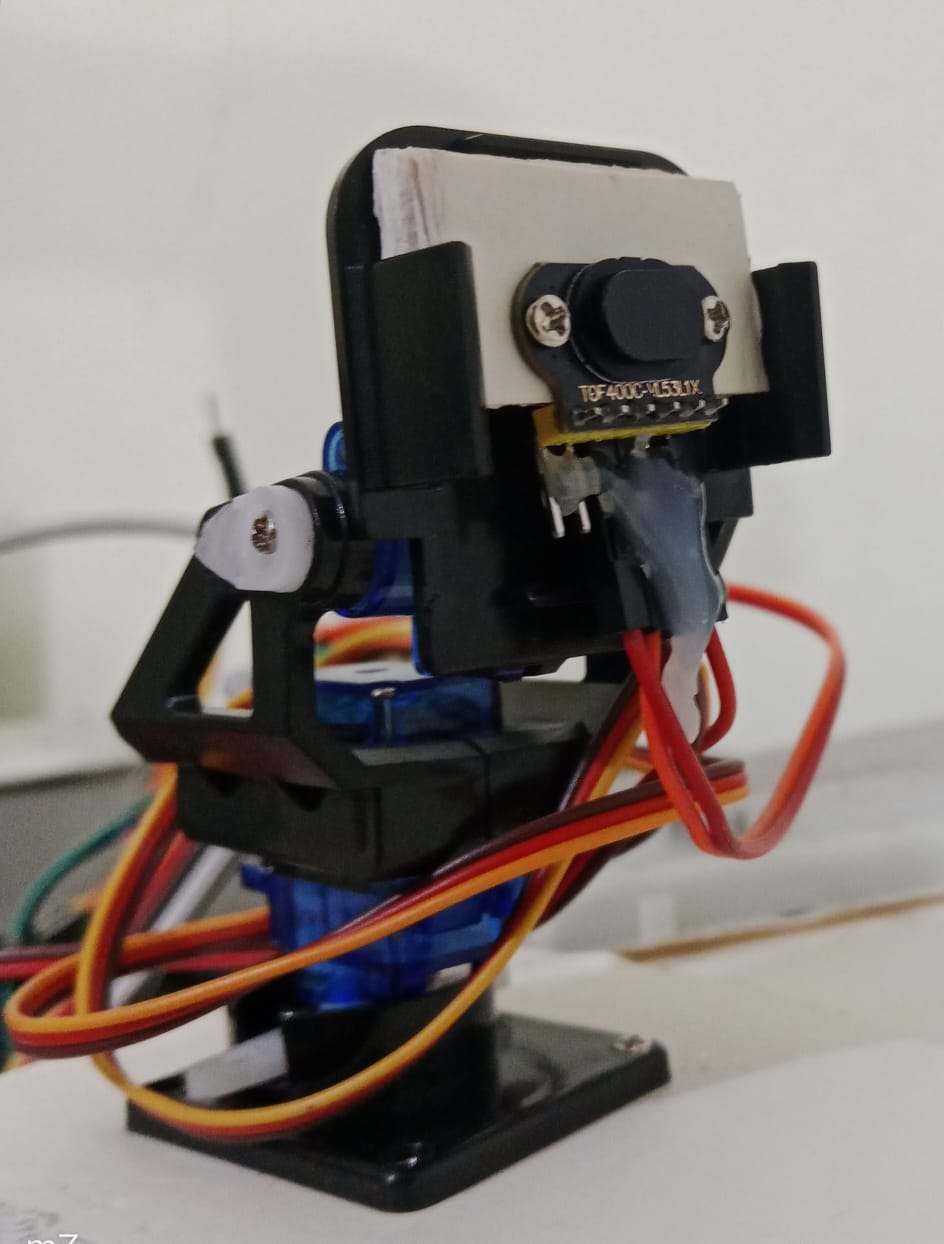
\includegraphics[width=0.8\columnwidth]{figures/TOF 400cVL53L1X sensor attached with 2 sg-90 servo.png}}
\caption{The assembled pan-tilt rig. A TOF400 (VL53L1X) module sits on two SG90 servos, wired directly to an ESP32 without external motor drivers.}
\label{fig:hardware}
\end{figure}

\subsection{Sensor and MCU}
The TOF400 breakout board carries the VL53L1X and communicates over $I^2C$ at 400~kHz. We connected it to an ESP32 DevKit running FreeRTOS and set the sensor's timing budget to 50~ms per measurement---a compromise between getting enough photon counts for accuracy and keeping the overall scan time reasonable.

\subsection{Pan-Tilt Mechanism}
Two SG90 micro servos handle azimuth and elevation (Fig.~\ref{fig:hardware}). We drove them straight from the ESP32's LEDC PWM channels, but powered them off a separate 5~V rail. Trying to run them from the ESP32's onboard regulator caused brownouts within the first five minutes of scanning---a lesson learned the hard way.

\subsection{Environmental Logging}
A DHT11 temperature sensor and an INA219 current monitor were added to track ambient conditions during each scan session. The DHT11 is far from laboratory-grade, but it gives us enough resolution to flag any thermal drift in the VCSEL emitter. The INA219 catches power sags that might affect servo positioning.

\section{Error Model and Ground Truth}

\subsection{Coordinate Transform}
Each raw range $r$ at pan angle $\theta$ and tilt angle $\phi$ maps to Cartesian space via the standard spherical transform:
\begin{align}
x &= r \cos \theta \cos \phi \nonumber \\
y &= r \sin \theta \cos \phi \label{eq:spherical} \\
z &= r \sin \phi \nonumber
\end{align}

The spherical mapping reveals how angular errors propagate into Cartesian space. For small angular errors, lateral displacement scales with distance: $\Delta x \approx r\Delta\theta$. At 3~m range, a 0.25$^\circ$ angular error from servo jitter translates to approximately 13.1~mm of lateral displacement. This is why we put so much effort into ground truth.

\begin{figure}[htbp]
\centerline{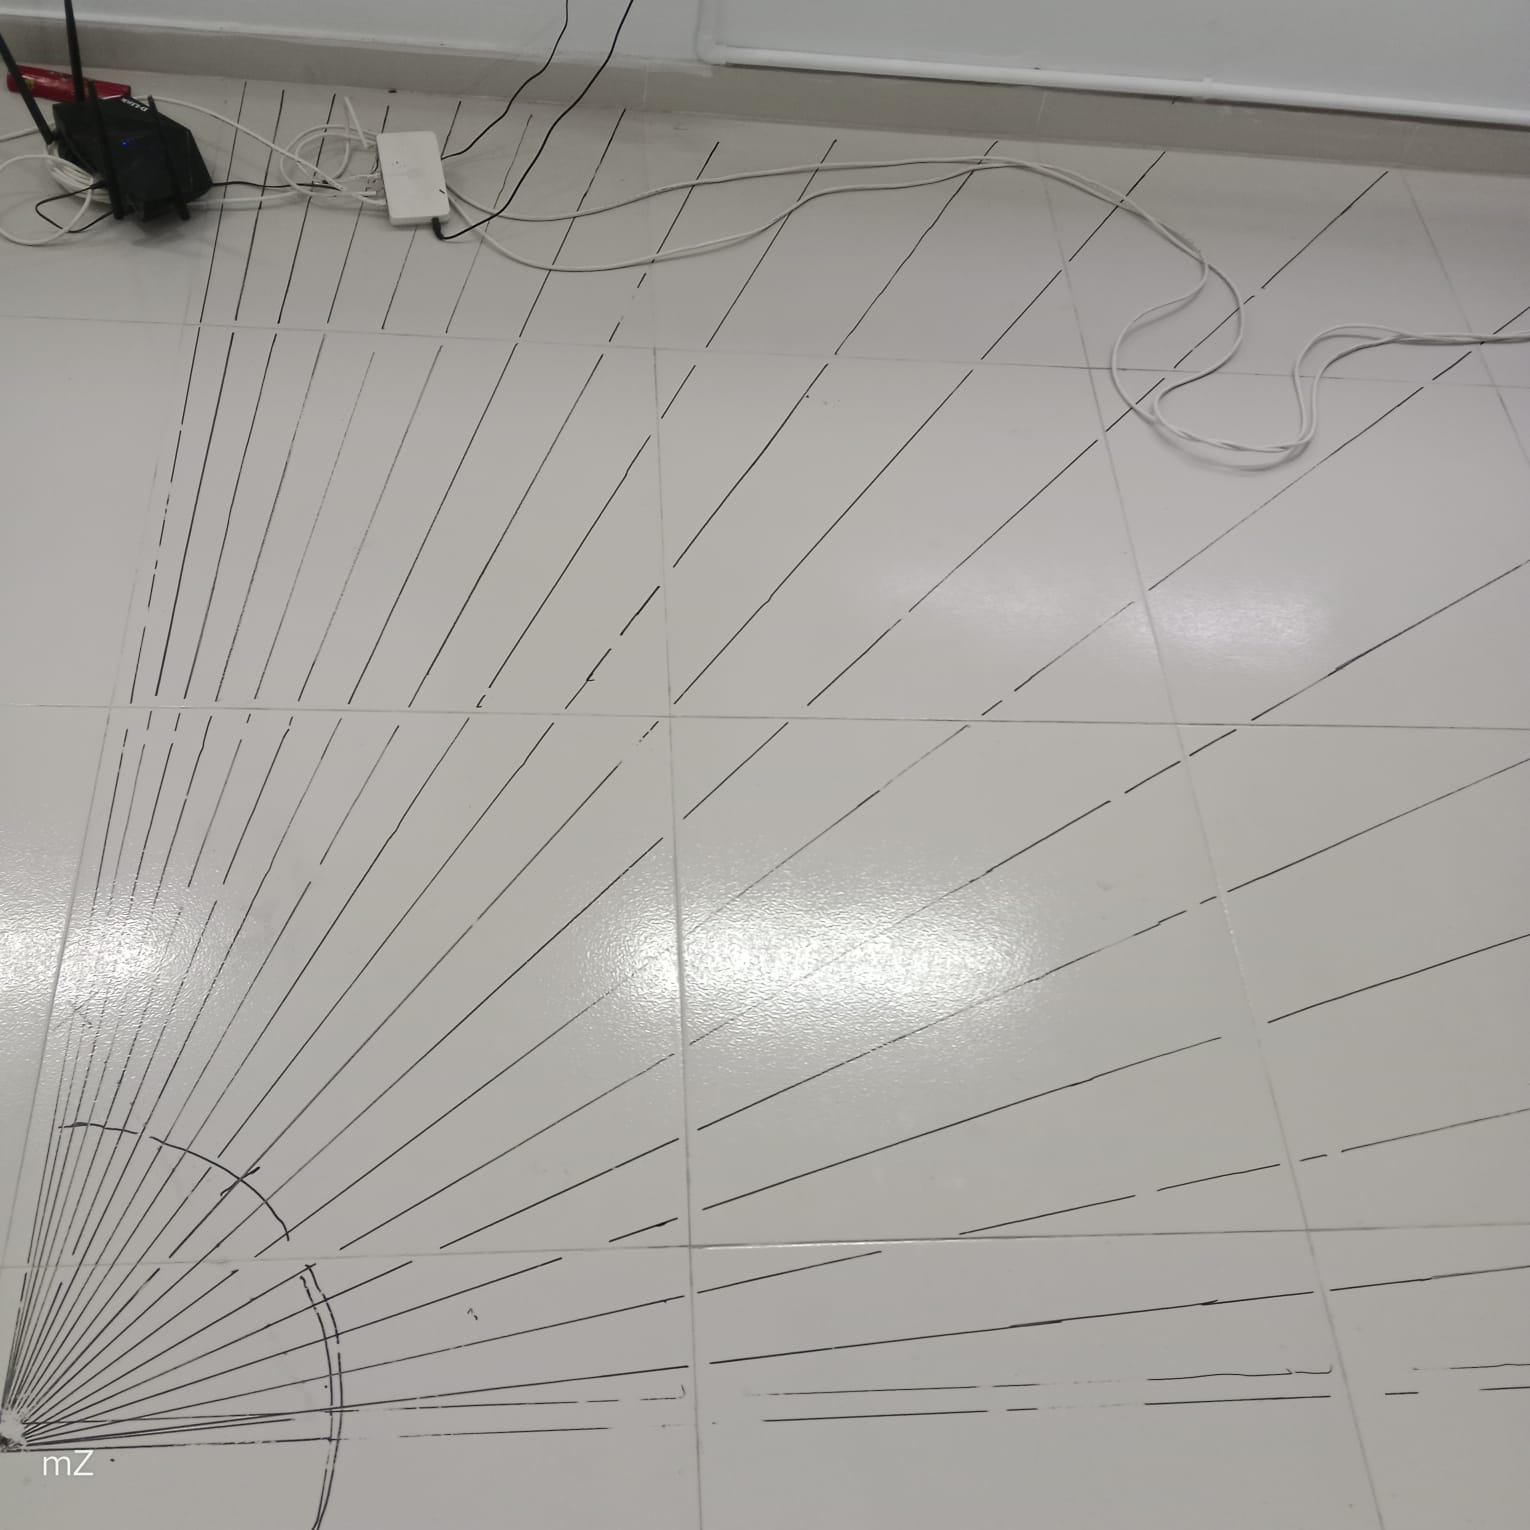
\includegraphics[width=\columnwidth]{figures/Ground truth measuring.png}}
\caption{Ground-truth setup. A large protractor grid taped to the floor defines angular reference lines; walls and boxes are measured with a tape and laser measure.}
\label{fig:groundtruth_setup}
\end{figure}

\subsection{How We Built the Dataset}
We did not have access to a reference-grade LiDAR, so we derived ground truth geometrically. The pan-tilt rotation center sat at the origin of a floor protractor (Fig.~\ref{fig:groundtruth_setup}). Walls and boxes were measured by hand, and at every pan/tilt step the expected range $r_{GT}$ was computed as a ray--plane intersection. The geometric ground truth provides a controlled reference derived from measured planar surfaces; its uncertainty is dominated by surface measurement, alignment, and servo-angle errors. The study evaluates calibration against geometry-derived references rather than an independent metrology-grade range instrument. Future work will validate the method against a reference LiDAR and under variable illumination conditions.

\begin{figure}[htbp]
\centerline{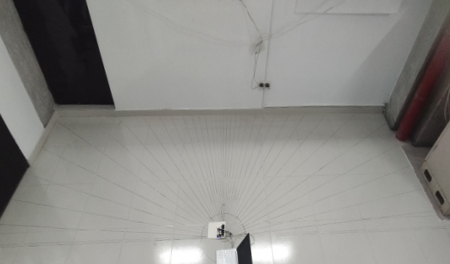
\includegraphics[width=\columnwidth]{figures/scanning the ground truth area.png}}
\caption{The scanner mid-sweep. Each session covered pan angles 0--180$^\circ$ and tilt angles 95--170$^\circ$ at 1$^\circ$ pan steps.}
\label{fig:scanning}
\end{figure}

We ran ten separate scanning sessions (Fig.~\ref{fig:scanning}), yielding 57,352 data points in total. All retained measurements contained valid signal-rate, ambient-rate, and sigma telemetry; after filtering invalid range returns, 51,061 samples remained for model development. The room temperature drifted between 32$^\circ$C and 37$^\circ$C across sessions, which is realistic for an un-air-conditioned lab in a tropical climate. The tilt angle is defined relative to the servo's mechanical zero; therefore the 95$^\circ$--170$^\circ$ range corresponds to the downward-facing scanning region. This is wide enough to avoid single-angle bias.

Fig.~\ref{fig:rawvsgt} plots every measurement against its ground truth. The bulk of the data hugs the ideal 1:1 line, but look at the scatter beyond 2,500~mm---that is exactly where multipath and weak returns start to bite, and exactly where we expect the ML model to help.

\begin{figure}[htbp]
\centerline{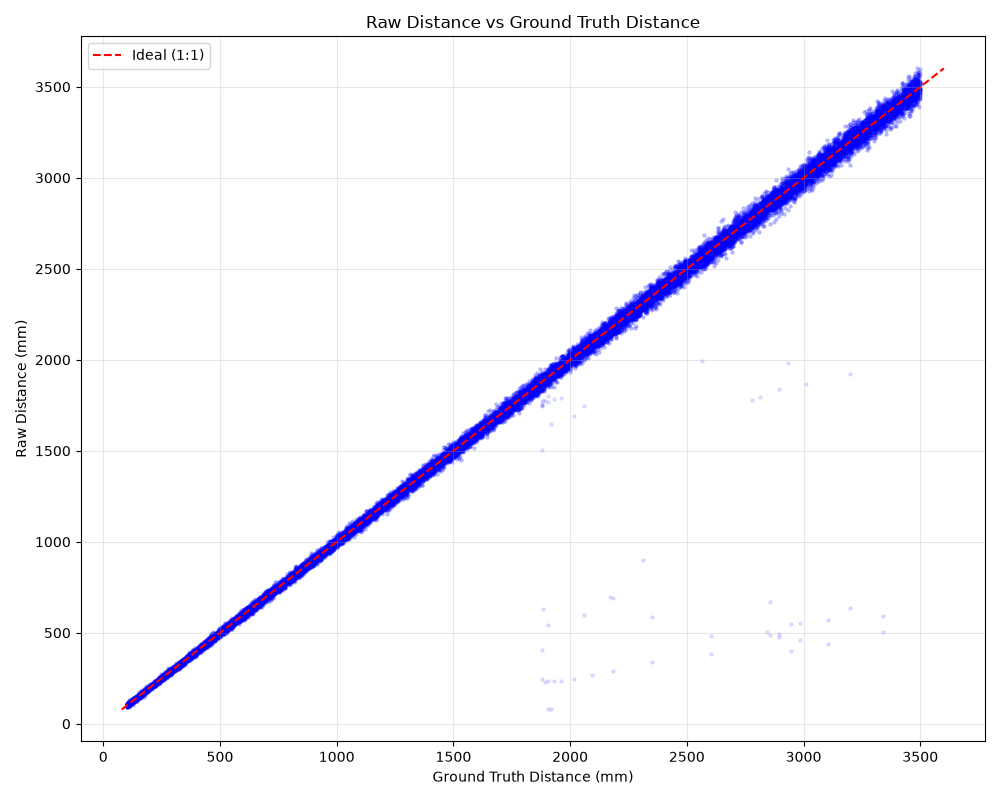
\includegraphics[width=\columnwidth]{figures/raw_vs_gt.png}}
\caption{Raw distance vs.\ ground truth for all 57,352 points. Most readings follow the ideal diagonal (red dashed), but outliers grow at longer ranges---the pattern our model needs to learn.}
\label{fig:rawvsgt}
\end{figure}

\section{ML Approach}

\subsection{Predicting the Residual, Not the Distance}
A naive approach would be to train a model that takes the six input features and outputs the ``correct'' distance. We tried this early on, and the model essentially memorized the identity function $\hat{r} \approx r_{raw}$ while ignoring the signal features. It optimized the wrong thing.

Instead, we trained the model on the residual:
\begin{equation}
e_i = r_{GT,i} - r_{raw,i}
\end{equation}
and applied the correction as $r_{corr} = r_{raw} + \hat{e}$. This forces the model to focus on what the sensor gets wrong, not on what it already gets right. The feature vector for each sample is:

\begin{itemize}
    \item \textbf{$r_{raw}$}: raw distance in mm.
    \item \textbf{$\theta$, $\phi$}: pan and tilt angles, capturing positional distortion.
    \item \textbf{Signal Rate} (kcps): strength of the reflected laser return.
    \item \textbf{Ambient Rate} (kcps): background IR noise level.
    \item \textbf{Sigma} (mm): the VL53L1X's own confidence estimate.
\end{itemize}

The full inference pipeline is sketched in Fig.~\ref{fig:architecture}. Fig.~\ref{fig:correlation} confirms that several of these features, particularly signal and ambient rate, do in fact correlate with the residual error---which is the whole premise of our ``signal-aware'' approach.

\begin{figure}[htbp]
\centering
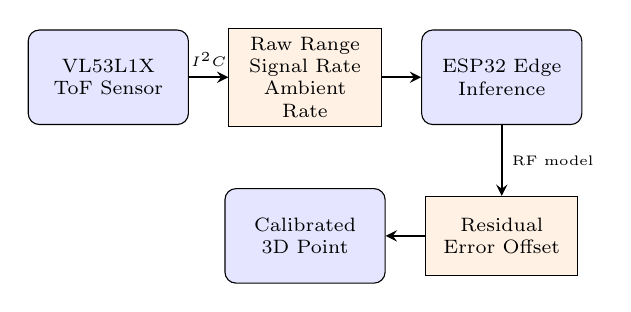
\begin{tikzpicture}[
    node distance=0.9cm and 0.5cm,
    block/.style={rectangle, draw, fill=blue!10, text width=1.8cm, text centered, rounded corners, minimum height=1.2cm, font=\scriptsize},
    data/.style={rectangle, draw, fill=orange!10, text width=1.7cm, text centered, minimum height=1cm, font=\scriptsize},
    arrow/.style={thick,->,>=stealth}
]

\node [block] (sensor) {VL53L1X\\ToF Sensor};
\node [data, right=of sensor] (features) {Raw Range\\Signal Rate\\Ambient Rate};
\node [block, right=of features] (esp) {ESP32 Edge\\Inference};
\node [data, below=of esp] (error) {Residual\\Error Offset};
\node [block, left=of error] (calib) {Calibrated\\3D Point};

\draw [arrow] (sensor) -- node[above, font=\tiny] {$I^2C$} (features);
\draw [arrow] (features) -- (esp);
\draw [arrow] (esp) -- node[right, font=\tiny] {RF model} (error);
\draw [arrow] (error) -- (calib);

\end{tikzpicture}
\caption{Inference pipeline. Sensor telemetry flows over $I^2C$ to the ESP32, which runs the transpiled Random Forest and applies the correction before computing Cartesian coordinates.}
\label{fig:architecture}
\end{figure}

\begin{figure}[htbp]
\centerline{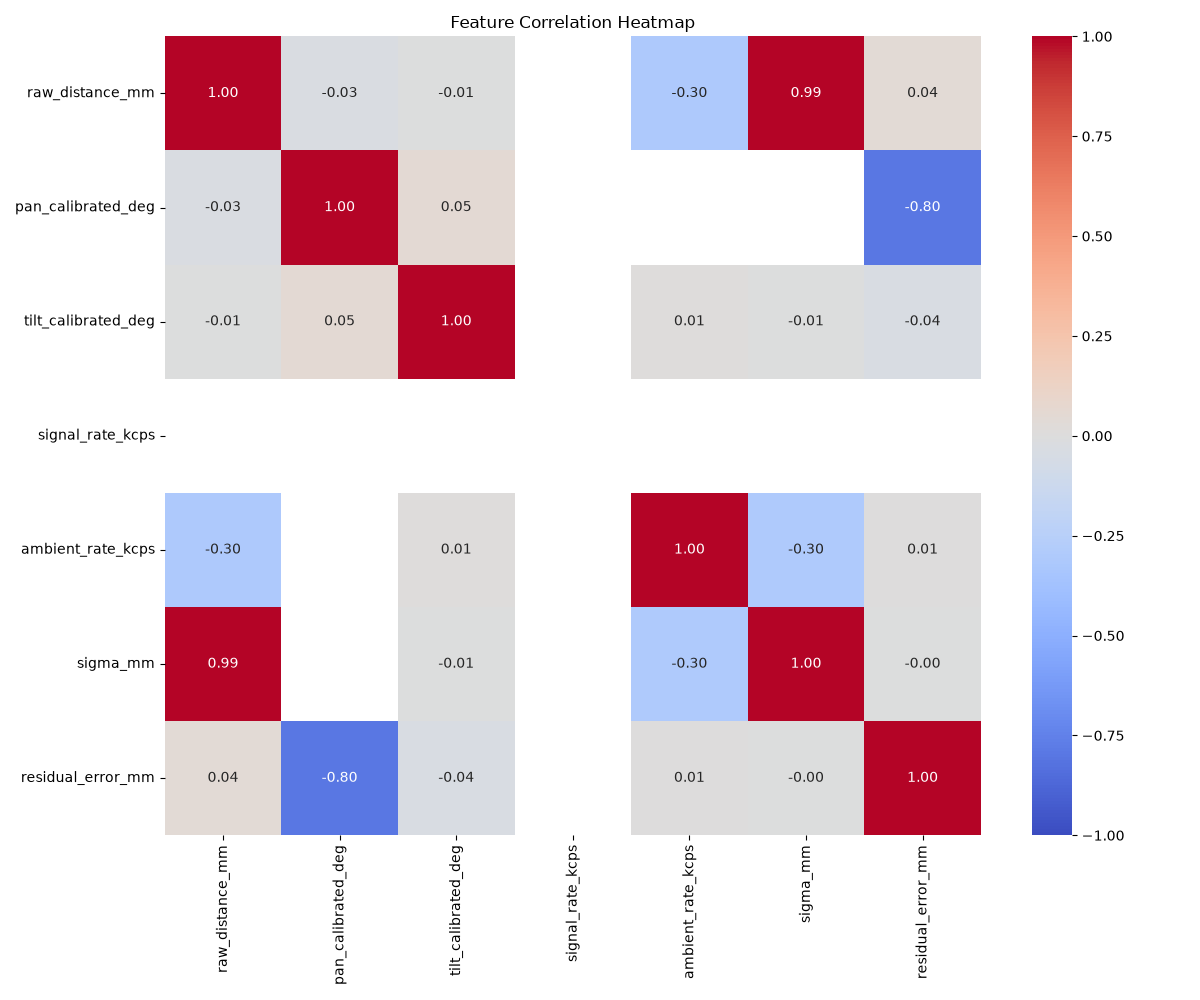
\includegraphics[width=0.9\columnwidth]{figures/feature_correlation.png}}
\caption{Correlation heatmap. Signal and ambient rates show meaningful correlation with the residual error, justifying their inclusion as model features.}
\label{fig:correlation}
\end{figure}

\subsection{Model Selection}
After filtering out invalid returns, we had 51,061 usable samples. We randomly held out 20\% of individual measurements for testing (i.e., a sample-level split rather than a session-level split) and trained three model families: ordinary least-squares linear regression, Random Forest \cite{breiman2001random}, and XGBoost \cite{chen2016xgboost}.

We deliberately skipped deep neural networks. A small MLP might have worked accuracy-wise, but deploying one on an ESP32 requires either TensorFlow Lite Micro (which eats most of the available Flash) or a custom inference loop with hand-tuned fixed-point weights. Tree ensembles offered a much cleaner path to the microcontroller.

\section{Results}

\subsection{Accuracy}
Table~\ref{tab:accuracy} tells the story. The raw sensor baseline sat at 18.37~mm MAE. Linear regression barely moved the needle (18.01~mm)---not surprising, since the errors are non-linear. Both tree-based models did better. XGBoost squeezed out the lowest MAE at 16.99~mm, and the Random Forest was close behind at 17.35~mm.

\begin{table}[htbp]
\caption{Calibration Results on the Held-Out Test Set}
\begin{center}
\begin{tabularx}{\columnwidth}{>{\raggedright\arraybackslash}X >{\centering\arraybackslash}X >{\centering\arraybackslash}X}
\toprule
\textbf{Model} & \textbf{MAE (mm)} & \textbf{95th Pct. (mm)} \\
\midrule
Raw Sensor Baseline & 18.37 & 53.37 \\
Linear Regression & 18.01 & 51.30 \\
Random Forest (Edge) & 17.35 & 49.08 \\
XGBoost (Best) & \textbf{16.99} & \textbf{48.80} \\
\bottomrule
\end{tabularx}
\label{tab:accuracy}
\end{center}
\end{table}

The more interesting number is the 95th-percentile column. Worst-case errors dropped from 53.37~mm to 49.08~mm with the Random Forest---a 4.3~mm reduction in the tail. For a system destined for obstacle avoidance or room mapping, pulling in those outliers matters more than shaving a millimeter off the average. The error distribution shift is visible in Fig.~\ref{fig:distribution}.

\begin{figure}[htbp]
\centerline{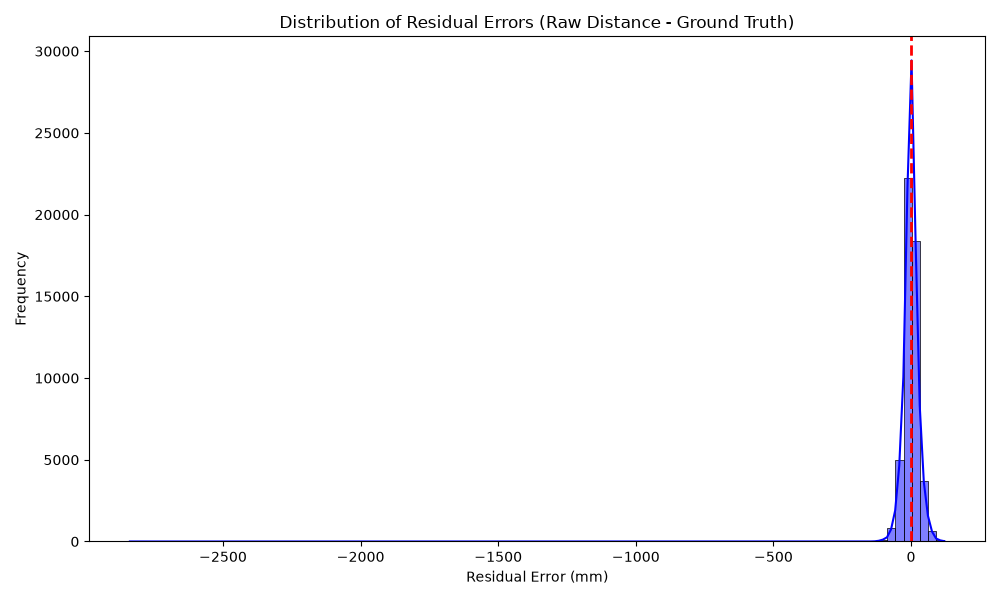
\includegraphics[width=\columnwidth]{figures/error_distribution.png}}
\caption{Residual error distribution before and after calibration. The ML-corrected curve is narrower and more tightly centered around zero.}
\label{fig:distribution}
\end{figure}

\subsection{What the Model Actually Learned}
Fig.~\ref{fig:importance} breaks down feature importance for the tree ensembles. Raw distance dominates---which makes sense, since the magnitude of the error obviously scales with range. But signal rate and ambient rate carry real weight too. The feature-importance results indicate that the model uses photon-return context in addition to raw distance to modulate its correction.

\begin{figure}[htbp]
\centerline{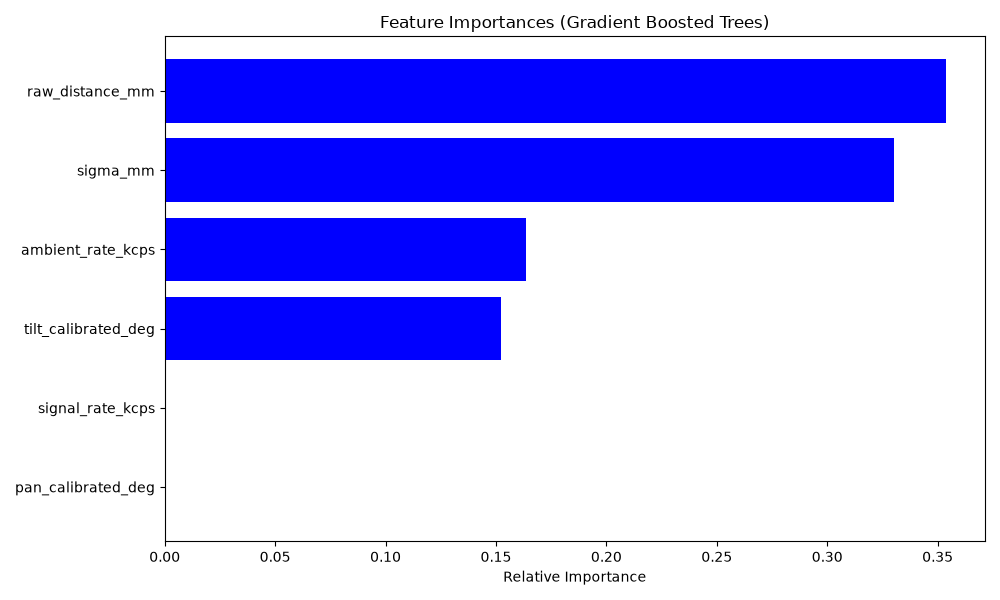
\includegraphics[width=\columnwidth]{figures/feature_importance.png}}
\caption{Feature importance from the trained ensemble. Signal and ambient rates carry meaningful predictive weight beyond raw distance alone.}
\label{fig:importance}
\end{figure}

\subsection{Getting the Model onto the ESP32}
We used \texttt{m2cgen} (``model to code generation'') to convert the trained Random Forest into a single C++ function---roughly 70,000 lines of nested \texttt{if-else} blocks. No runtime library, no dynamic memory, just comparisons and floating-point constants baked into Flash.

Compilation takes about 15--20 minutes on a modern laptop (the GCC optimizer chews through all those branches), but the result is worth the wait. On the ESP32, each inference call finishes in under 100~$\mu$s. Inference latency was measured using ESP32 hardware timer instrumentation over repeated predictions, excluding $I^2C$ acquisition. Since the VL53L1X itself needs 50~ms to complete a ranging cycle, the ML overhead is invisible---it fits entirely inside the sensor's own dead time.

Why not deploy the more accurate XGBoost model? We tried. Its deeper trees produced an even larger C file that pushed past the ESP32's 3~MB Flash partition. The Random Forest gave up just 0.36~mm of MAE in exchange for a much smaller binary. We considered that a reasonable trade-off.

\subsection{3D Reconstruction}
Numbers aside, the real test is whether the corrected ranges produce cleaner geometry. Fig.~\ref{fig:cloud1} and Fig.~\ref{fig:cloud2} show the resulting point clouds from two perspectives. Wall planes are flatter, object edges are tighter, and there are fewer stray points floating in mid-air. It is not a dramatic before-and-after---the raw sensor was already quite good indoors---but the structural improvement is visible.

\begin{figure}[htbp]
\centerline{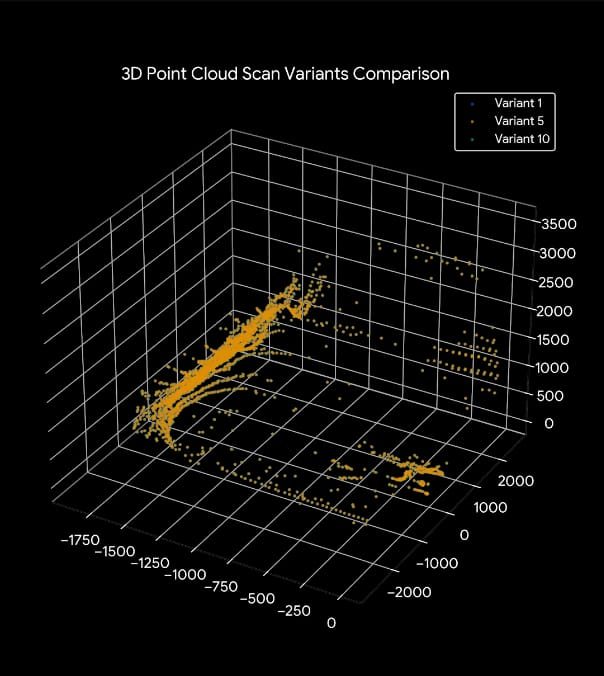
\includegraphics[width=\columnwidth]{figures/3D Cloud point Mapping-1.png}}
\caption{Reconstructed 3D point cloud of the test environment, viewed from above. Structural outlines of walls and furniture are clearly resolved.}
\label{fig:cloud1}
\end{figure}

\begin{figure}[htbp]
\centerline{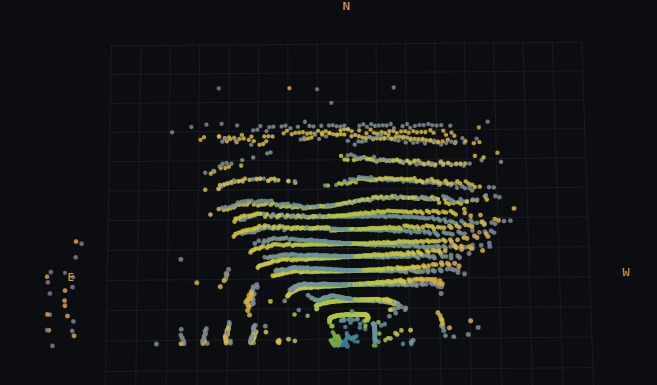
\includegraphics[width=\columnwidth]{figures/Cloud point Mapping.png}}
\caption{A second viewpoint of the same scan, showing depth layering between foreground objects and the back wall.}
\label{fig:cloud2}
\end{figure}

\subsection{Where It Breaks Down}
We would be dishonest if we did not mention the failure cases. On matte black fabric, the signal rate dropped so low that it was essentially indistinguishable from noise---the model had nothing useful to work with. Glass and mirrors were even worse: specular reflections sent the photon counts haywire, and the tree ensembles produced corrections that were sometimes larger than the original error. Any deployment of this system in a real robot would need a fallback path (ultrasonic, perhaps) for those edge cases.

\section{Conclusion}
We set out to test whether a low-cost ToF sensor could be taught to correct its own errors using nothing but its internal signal telemetry and an ESP32 microcontroller. The answer is a qualified yes. The ML model learns real structure in the residuals---it is not just curve-fitting against distance---and it runs comfortably within the ESP32's resource envelope.

The gains in our controlled indoor setup were modest (roughly 1~mm on average, 4~mm at the 95th percentile), because the raw sensor was already performing well. The more compelling scenario is outdoors or in challenging reflectivity conditions, where raw ToF errors can balloon to 20--50~cm. We expect the signal-aware approach to pay off much more dramatically there, and that is the direction of our ongoing work.

All source code, training scripts, the ESP32 firmware, and the LaTeX source for this paper will be made publicly available upon publication.

\bibliographystyle{IEEEtran}
\bibliography{references}

\end{document}
